\documentclass[prl,twocolumn]{revtex4-1}

\usepackage{graphicx}
\usepackage{color}
\usepackage{latexsym,amsmath}
\usepackage{amsfonts}
\usepackage{caption}
\usepackage{siunitx}
\usepackage{mathtools}

\definecolor{linkcolor}{rgb}{1.0,0.647,0.0} %hyperlink
\usepackage[pdftex,colorlinks=true, pdfstartview=FitV, linkcolor= linkcolor, citecolor= linkcolor, urlcolor= linkcolor, hyperindex=true,hyperfigures=true]{hyperref} %hyperlink%

\usepackage{enumitem}
\setlist[itemize]{leftmargin=*}


\setcounter{secnumdepth}{2}

\renewcommand{\thesection}{\arabic{section}}
\renewcommand{\theequation}{\thesection.\arabic{equation}}

\makeatletter
\@addtoreset{equation}{section} % Reset equation counter at each section
\makeatother

\begin{document}

\title{Quantum Optics and Laser - Final essay \\ **** \\ \Large{Pumping schemes and pumping technology. \\Ranges of optical gain and applications in the different spectral regions.}}



\author{Calandra Buonaura Lorenzo}

\date{\today}

\begin{abstract}
This essay explores the role of the main pumping schemes in laser systems, analyzing their optical gain characteristics. Different implementations across some spectral regions are examined, presenting the main characteristics and applications.
\end{abstract}

\maketitle

\section{Laser Amplifiers}
The fundamental principles of laser amplifiers are rooted in the three primary interactions between photons and atoms: absorption, stimulated emission, and spontaneous emission. These processes form the foundation of light amplification, where stimulated emission plays a pivotal role in amplifying the intensity of light within the laser medium. 

Consider a photon with frequency $\nu$ interacting with an atom in its ground state. The interaction can result in the absorption of the photon or in the emission of another photon with identical frequency, phase, and direction; these processes are characterized by their respective probability densities. The probability density that an unexcited atom absorbs a single photon is given by~\cite{Saleh2007}:
%
\begin{equation}
    \label{eq:probability_density}
    W_i = \sigma(\nu) \Phi,
\end{equation}
%
where $\sigma(\nu)$ is the transition cross section at the frequency $\nu$ and $\Phi$ is the photon flux. The probability density for stimulated emission is identical to that for absorption. The transition cross section depends on the normalized lineshape function ($g(\nu)$, the effective spontaneous lifetime for stimulated emission ($t_{sp}$), and the wavelength of light in the medium ($\lambda$) through a specific relation~\cite{Saleh2007}:  
%
\begin{equation}
    \sigma(\nu) = \frac{\lambda^2}{8 \pi t_{sp}} g(\nu).
\end{equation}

The average density of absorbed photons (number of photons per unit time per unit volume) is $N_1 W_i$ and, similarly, the average density of clone photons generated due to stimulated emission is $N_2 W_i$. The net number of photons gained per second per unit volume is therefore $N W_i$, where:
%
\begin{equation}
    \label{eq:population_difference}
    N = N_2 - N_1
\end{equation}
%
is the population density difference, often referred to as the population difference. We can have three regimes:
\begin{itemize}
    \item \textbf{$N>0$:} a \textit{population inversion} exists, the medium acts as an amplifier, and the photon-flux density of a wave passing through it increases.
    \item \textbf{$N<0$:} the medium acts as an attenuator, reducing the photon-flux density.
    \item \textbf{$N=0$:} the medium is transparent.
\end{itemize}

Considering that in our reference system the incident photons travel in the $z$ direction, the stimulated emission photons also travel in that direction; since emitted photons stimulate further emissions, the growth at any position z is proportional to the population at that position and thus $\Phi(z)$ increases exponentially. This can be easily proved considering the differential equation:
%
\begin{equation}
    \frac{d\Phi(z)}{dz} = \gamma(\nu) \Phi(z),
\end{equation}
%
where $\gamma(\nu) = N \sigma(\nu)$ is the net gain coefficient. Consequently, the solution to the differential equation is:
%
\begin{equation}
    \Phi(z) = \Phi(0) \exp[\gamma(\nu) z].
\end{equation}

Since the optical intensity $I(z) = h \nu \Phi(z)$, the equation can also be written in terms of intensity; thus, $\gamma(\nu)$ represents the gain in intensity per unit length of the medium.

The overall gain $G(\nu)$ of the amplifier for an interaction region of length $d$ is then given by~\cite{Saleh2007}:
%
\begin{equation}
\label{eq:optical_gain}
    G(\nu) = \frac{\Phi(d)}{\Phi(0)} = e^[\gamma(\nu) d].
\end{equation}

The dependence of $\gamma(\nu)$ on the frequency of incident light is determined by the lineshape function $g(\nu)$, which is centered around the resonance frequency $\nu_0 = \frac{E_2 - E_1}{h}$ with a linewidth \(\Delta \nu\).

Like other amplifiers, laser amplifiers require an external source of power to provide the energy required to augment the input signal: the pump supplies this power via a mechanism that excites the electrons in the atoms, causing them to move from lower to higher atomic energy levels. As already pointed out, to achieve amplification, the pump must provide a population inversion on the transition of interest (so that $N > 0$). To attain the continuous-wave (CW) operation of a laser amplifier, the rates of excitation and decay of the various energy levels participating in the process must be balanced to maintain a steady-state inverted population on $2 \rightarrow 1$ transition~\cite{Siegman1986}. 

\section{Pumping Schemes}
In this section we take in consideration the most important pumping schemes, highlighting why and how the mechanics of pumping often involves the use of ausiliary energy levels.

\subsection{Two-level pumping}

\begin{figure}[!b]
    \centering
    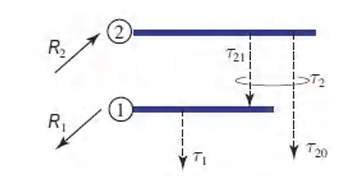
\includegraphics[width=0.7\linewidth]{Images/two_level_scheme.png}
    \caption{Two-level pumping scheme, with decay times. By means of pumping, the population density of level 2 is increased at the rate $R_2$ while that of level 1 is decreased at the rate $R_1$~\cite{Saleh2007}.}
    \label{fig:two_level_scheme}
\end{figure}

In a two-level pumping scheme, we consider a two-level atomic system (1 and 2, with population densities $N_1$ and $N_2$, respectively): external energy is supplied to atoms initially in the lower energy state 1, exciting them to the upper energy state 2 (see Figure~\ref{fig:two_level_scheme}). The goal of this process is to achieve a population inversion, which we have shown to be a necessary condition for amplification by stimulated emission; however, the two-level scheme faces intrinsic limitations that prevent population inversion.

Moreover, we must remember that the behavior of the atomic system changes depending on whether there is an external electromagnetic radiation present at the resonance frequency of the transition between the two levels: we can thus identify two cases, with or without amplifier radiation, meaning with or without the resonant external field~\cite{Saleh2007}.

\subsubsection{\textbf{Rate equations without amplifier radiation}}
In order to study the population difference of a scheme, we must solve a system of coupled equations that express the population variations due to pumping and decay. In the case of a 2-level pumping scheme, in absence of amplifier radiation, these equations look like:
%
\begin{equation}
    \begin{dcases}
        \frac{dN_2}{dt} = R_2-\frac{N_2}{\tau_2} \\
        \frac{dN_1}{dt} = -R_1-\frac{N_1}{\tau_1}+\frac{N_2}{\tau_{21}}
    \end{dcases}
    \label{eq:rate_equations_two_levels}
\end{equation}
%
%
where $R_1$ and $R_2$ are the pumping rates for the two levels (per unit volume per unit time), $\tau_1$ and $\tau_2$ are the lifetimes of the two levels and $\tau_{21}$ is the decay time for transitions from $2 \to 1$~\cite{Saleh2007}.

Under steady-state conditions (both fluxes are null), these equation can be solved and we obtain that the population difference (Equation~\eqref{eq:population_difference}), in the absence of amplifier radiation, is given by:
%
\begin{equation}
    \label{eq:N_0_without}
    N_0 = \frac{\tau_2 R_2 - \tau_1 R_1}{1 + \tau_2 R_2 / \tau_{21}},
\end{equation}
%

For $R_1 = 0$ (no depumping from $1$) and assuming that level 1 is a short lived state ($\tau_1 \ll \tau_{21}$), the population difference simplifies to:
%
\begin{equation}
N_0 \approx R_2 \tau_2.
\end{equation}  

\subsubsection{\textbf{Rate equations with amplifier radiation}}
In the presence of resonant amplifier radiation, we must modify the rate equations (Equation~\eqref{eq:rate_equations_two_levels}) in order to account for stimulated absorption and emission, which occur with identical rates, given by Equation~\eqref{eq:probability_density}. Then, the population difference becomes~\cite{Saleh2007}:
%
\begin{equation}
    \label{eq:N_with}
    N = \frac{N_0}{1 + \tau_s W_i},
\end{equation}
%
where $N_0$ is the steady-state population difference in the absence of amplifier radiation (Equation~\eqref{eq:N_0_without}) and $\tau_s$ is the saturation time constant:
%
\begin{equation}
    \label{eq:saturation_time}
    \tau_s = \tau_2+ \tau_1\left(1-\frac{\tau_2}{\tau_{21}}\right)
\end{equation} 

\subsubsection{\textbf{Limitations}}
In the first case, without amplifier radiation, the population difference is $N = N_0$, which can achieve a steady positive value, enabling the potential for optical gain (even if $N_0$ is usually a small value). However, in the second case, when amplifier radiation is present (most of the cases), the population difference is reduced to Equation~\eqref{eq:N_with}: as $W_i$ increases, $N$ approaches zero, making population inversion ($N_2 > N_1$) impossible in a two-level system. This result demonstrates that a two-level pumping scheme cannot maintain a population inversion in the presence of amplifier radiation, because stimulated absorption and emission processes occur at equal rates, and their balance nullifies the population difference required for amplification~\cite{Saleh2007}. 

\subsection{Three-level pumping}

We have shown that in a two-level system, any pumping process involving amplifier radiation simultaneously increases the stimulated absorption rate. Consequently, population inversion cannot be achieved and so this limitation necessitates the use of three-level or four-level systems for practical laser operation, where additional energy levels decouple the absorption and emission processes.

\begin{figure}[!t]
    \centering
    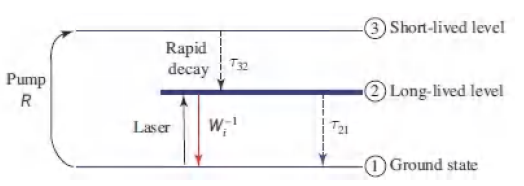
\includegraphics[width=0.9\linewidth]{Images/three_level_scheme.png}
    \caption{Energy levels and decay rates for a three-level system. We assume that the rate of pumping into level 3 is the same as the rate of pumping out of level 1~\cite{Saleh2007}.}
    \label{fig:three_level_scheme}
\end{figure}

A three-level pumping arrangement makes use of the ground state $E_1 = 0$ as the lower laser level and an auxiliary third level is involved, characterized by a rapid decay (no population buildup). The decay from level $2$ is slow ($\tau_{32} \ll \tau_{31}$), allowing the pumping process to populate it (long-lived upper level). How does the scheme work? Atoms are pumped from the ground state to level $3$ (by absorbing light at frequency $\nu \approx E_3/h$) at a rate $R$; the rapid (nonradiative) decay effectively pumps level $2$ at a rate $R_2 = R$, while the thermally excited population of level $E_3$ is assumed to be negligible (see Figure~\ref{fig:three_level_scheme}). This correspond to a special case of the system in Figure~\ref{fig:two_level_scheme}, where $R_1=R_2=R$, $\tau_1=\infty$ and $\tau_2=\tau_{21}$. 

\subsubsection{\textbf{Population difference with amplifier radiation}}

Given the previous argument, we can solve the rate equations with amplifier radiation (which previously led to Equation~\eqref{eq:N_with}) also in this case. Due to $R_1=R_2$, both equations give the same result, so we can solve the system introducing the total atomic density $N_a$ in the levels; since level 3 is a short-lived states, we have that:
%
\begin{equation}
\label{eq:pop_density}
N_1 + N_2 \approx N_a,
\end{equation}
%
which enables us to solve for $N_1$ and $N_2$ and thereby determine the population difference $N$ and the saturation time $\tau_s$. The result may be cast in the same form of Equation~\eqref{eq:N_with}, where now~\cite{Saleh2007}:
%
\begin{equation}
N_0 = 2R \tau_{21} - N_a \quad \quad \tau_s = 2\tau_{21}.
\end{equation}

\subsubsection{\textbf{Population difference without amplifier radiation}}

When nonradiative decay from level $2$ to $11$ is negligible, $\tau_{21}$ may be replaced by $t_{sp}$, yielding:
%
\begin{equation}
\label{eq:results_three}
N_0 \approx 2R t_{sp} - N_a \quad \quad \tau_s \approx 2t_{sp}.
\end{equation}

Implicit in the preceding derivation is the assumption that the pumping rate $R$ is independent of the population difference $N$~\cite{Saleh2007}. This is not always the case, however, because the population densities are related by Equation~\eqref{eq:pop_density}. If the pumping involves a transition between the ground state and level $3$ with transition probability W, then the dependence of the pumping rate $R$ on the population difference $N$ can be included by writing:
%
\begin{equation}
R = (N_1 - N_3) W \approx N_1W \quad \quad N_1 = \frac{1}{2} (N_a - N),
\end{equation}
%
from which we obtain:
%
\begin{equation}
R \approx \frac{1}{2} (N_a - N) W,
\end{equation}
%
which reveals that the pumping rate is a linearly decreasing function of the population difference $N$ and is thus clearly not independent of it. This arises because the population inversion established between levels $2$ and $1$ reduces the number of atoms available to be pumped.

Substituting this into the principal equation, we can write the population difference always like Equation~\eqref{eq:N_with}, but now with:
%
\begin{equation}
N_0 \approx \frac{N_a(t_{sp}W-1)}{1+t_{sp}W} \quad \quad \tau_s \approx \frac{2t_{sp}}{1+t_{sp}W}
\end{equation}
%
From these equations we can see that both $N_0$ and $\tau_s$ saturate as the pumping transition probability W increases; thus, also with amplifier radiation, is it possible to achieve population inversion with a three level scheme~\cite{Saleh2007}.


\subsection{Four-level pumping}
In a four-level pumping scheme, shown in Figure~\ref{fig:four_level_scheme}, level 1 lies above the ground state; in thermal equilibrium, this level will be virtually unpopulated provided that $E_1 \gg kT$, a situation that is, of course, desirable since it enhances the population inversion.

\begin{figure}[!t]
    \centering
    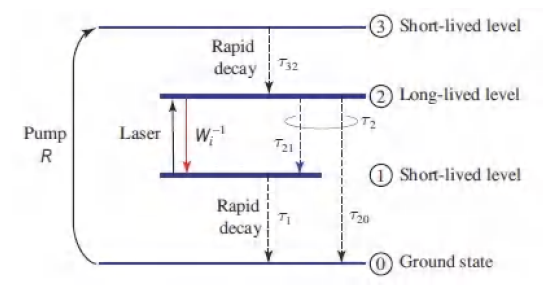
\includegraphics[width=0.9\linewidth]{Images/four_level_scheme.png}
    \caption{Energy levels and decay rates for a four-level system. The rate of pumping into level 3, and out of level 0, are taken to be the same. Level 1 is assumed to be unpopulated in thermal equilibrium. A quasi-three-level system has the same configuration except that level 1 is sufficiently close to level 0 that it retains population in thermal equilibrium~\cite{Saleh2007}.}
    \label{fig:four_level_scheme}
\end{figure}

Pumping is achieved by making use of an energy level that lies above level $2$; we designate this as level $3$. The $3 \to 2$ transition has a short lifetime, so there is little population accumulation in level $3$; level $2$ is long-lived, instead, so it accumulates population, whereas level $1$ is again short-lived; a population inversion is thereby established between levels $2$ and $1$. All told, four energy levels are involved in the process, but the optical interaction of interest takes place between levels $2$ and $1$~\cite{Saleh2007}.

How does the scheme work? An external source of energy (for example, photons at frequency $\nu \approx E_3/h$) pumps atoms from the ground state to level $3$ at a rate $R$. If the decay from level $3$ to level $2$ is sufficiently rapid, it may be taken to be instantaneous, which makes pumping to level $3$ is equivalent to pumping to level $2$ at the rate $R_2 = R$. The situation is then the same as that shown in Figure~\ref{fig:two_level_scheme}, so that Equation~\ref{eq:N_with} and Equation~\ref{eq:saturation_time} still apply. With respect to the value of $N_0$ to be used in these expressions, atoms are neither pumped into nor out of level $1$ in the four-level system, so $R_1 = 0$. In the absence of amplifier radiation ($W_i = \phi = 0$), therefore, the steady-state population difference is given by $N_0$, where:
%
\begin{equation}
    N_0 = R\: \tau_2 \left(1-\frac{\tau_2}{\tau_{21}}\right)
\end{equation}
%
In most four-level systems, the nonradiative decay component in the $2 \rightarrow 1$ transition is negligible, and $\tau_1 \ll t_{sp} \ll \tau_{20}$, so that
%
\begin{equation}
\label{eq:results_four}
N_0 \approx R \: t_{sp} \quad \quad \tau_s=t_{sp}
\end{equation}

Also in this case, implicit in the preceding derivation is the assumption that the pumping rate $R$ is independent of the population difference $N$. If we consider a pumping that involves a transition between the ground state and level $3$ with transition probability $W$, then

\begin{equation}
    R = (N_g - N_3)W\approx (N_a - N)W
\end{equation}
%
if levels $1$ and $3$ are short-lived, which again shows that the pumping rate is a linearly decreasing function of the population difference $N$. 
Substituting this into the principal equation, we can write the population difference always like Equation~\eqref{eq:N_with}, but now with:
%
\begin{equation}
    N_0 \approx \frac{R t_{sp} N_a}{1 + W t_{sp}} \quad \quad \tau_s \approx \frac{t_{sp}}{1 + W t_{sp}}.
\end{equation}

For weak pumping ($W \ll 1/t_{sp}$), $N_0 \approx t_{sp} N_a W$ is proportional to the pumping transition probability density $W$, and $\tau_s \approx t_{sp}$, so that the results obtained for the two-level scheme reemerge. However, also in this case, as the pumping strength increases, $N_0$ decreases and ultimately saturates, while $\tau_s$ decreases, so we obtain a population inversion~\cite{Saleh2007}.

\subsubsection{\textbf{Quasi-three-level pumping}}
Quasi-three-level pumping is a scheme intermediate between four-level
and three-level pumping. Its configuration is identical to that of four-level pumping (see Figure~\ref{fig:four_level_scheme}); the sole distinction is that the lower laser level (level $1$)is sufficiently close to the ground state that it retains some population in thermal equilibrium. As with the four-level system, pumping is achieved via auxiliary level $3$, the $3 \to 2$ transition is rapid, the
upper laser level $2$ is long-lived and a population inversion is established between levels $2$ and $1$ (which is short-lived).
However, because of the residual population in level $1$, reabsorption at the transition frequency makes the task of achieving a population inversion more challenging than in four-level pumping.

\subsection{Comparison of three- and four-level schemes}
It is of interest to compare the results for three-level pumping and for four-level pumping, derived in the previous section.

The first thing that can be noticed is that in order to obtain a population inversion ($N > 0$ and therefore $N_0 > 0$) in a three-level system we need a pumping rate 
%
\begin{equation}
    R > \frac{N_a}{2\tau_{sp}}.
\end{equation}
%
Thus, even to make the population density $N_2$ equal to $N_1$ (i.e., $N_0 = 0$), a substantial pump power density is required, given by 
%
\begin{equation}
\text{Pump power density} = \frac{E_3 N_a}{2\tau_{sp}}.
\end{equation}
%
This limitation arises because a significant fraction of the atomic population remains in the ground state (lower level of the scheme), requiring higher pump power to overcome.

In contrast, the four-level system avoids this impediment because the lower laser level is typically an intermediate energy state that is normally empty, as the decay time $\tau_1$ is short. This ensures that almost all the population is in the ground state, simplifying the achievement of a population inversion. Additionally, the saturation time constant for the four-level system (Equation~\eqref{eq:results_four}) is half of the saturation time constant for the three-level system (Equation~\eqref{eq:results_three}).

When considering the employment of these schemes, their use depends heavily on the requirements of the laser system and the properties of the lasing medium~\cite{Milonni2010}:

\begin{itemize}
    \item A three-level pumping scheme is often employed when simplicity is a key factor or when the energy level structure of the medium does not allow for a four-level configuration. For example, ruby lasers, which are based on a three-level system, have been successfully used despite their relatively high pump power requirements. However, achieving population inversion in such systems remains challenging.
    
    \item Four-level pumping schemes are preferred in applications where higher efficiency and lower pump thresholds are crucial. These systems are particularly suitable for continuous-wave operation since maintaining a population inversion is much easier. The absence of significant population in the lower laser level means that lasing can begin with minimal pump power, making these systems more efficient and versatile. A notable example of a four-level system is the Nd:YAG laser, which exhibits lower thresholds and greater operational efficiency compared to three-level systems.
    
    \item Quasi-three-level pumping schemes are used in systems where the lower laser level is thermally populated at room temperature, leading to some challenges in maintaining a population inversion. However, these schemes are employed when the material properties or energy level structures restrict the possibility of a true four-level system. Examples include Yb:YAG lasers, where the lower laser level lies just above the ground state. To reduce thermal population of the lower level, such lasers are often operated at cryogenic temperatures or with precise control over the pump wavelength to maximize efficiency.
\end{itemize}

\section{Pumping methods}
Many techniques are available for pumping laser amplifiers and lasers, the
most common of which make use of electrical and optical means (see Figure~\ref{fig:pumping_techniques}).

\begin{figure}[!b]
    \centering
    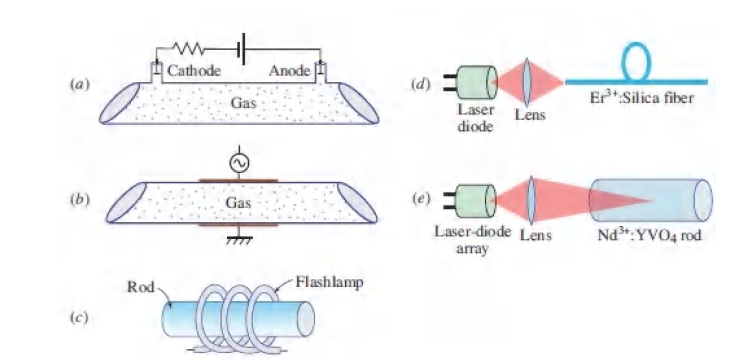
\includegraphics[width=\linewidth]{Images/pumping_techniques.png}
    \caption{Examples of electrical and optical pumping. \newline
    (a) Direct current (DC) pumping a gas laser. (b) Radio-frequency (RF) discharges are also used for pumping gas lasers. (c) Flashlamps can be used to optically pump ruby laser amplifiers and lasers. (d) Semiconductor laser diodes, which are themselves electrically pumped, are widely used for pumping $\text{Er}^{3+}$:silica-fiber laser amplifiers. (e) An array of laser diodes is generally used for the efficient optical pumping of $\text{Nd}^{3+}\text{:YVO}_4$ laser amplifiers and lasers~\cite{Saleh2007}.}
    \label{fig:pumping_techniques}
\end{figure}

\subsection{Optical pumping}
Optical pumping is a process in which light sources such as flashlamps, LEDs, or other lasers are used to transfer energy to the gain medium, exciting electrons to higher energy levels. The efficiency of optical pumping depends heavily on the spectral overlap between the emission spectrum of the pump source and the absorption bands of the gain medium~\cite{optical_pumping}.

\subsubsection{\textbf{Principle of optical pumping}}
The energy provided by the pump source corresponds to photons of a specific wavelength, $\lambda_p$, where the energy of the photons is given by:
%
\begin{equation}
    E_p = h \nu_p = \frac{hc}{\lambda_p},
\end{equation}
%
where $E_p$ is the energy of the pump photon and $\nu_p$ ($\lambda_p$) is the frequency (wavelength) of the pump light.

For population inversion to occur, the pump photons must have energies matching the energy difference between the ground state $1$ and an excited state $2$ in the gain medium, so this requires:
%
\begin{equation}
    \lambda_p \leq \frac{hc}{\Delta E}.
\end{equation}

\subsubsection{\textbf{Spectral overlap and efficiency}}
The overlap between the pump spectrum $S_p(\lambda)$ and the absorption spectrum $\alpha(\lambda)$ of the gain medium determines the pumping efficiency. This overlap can be quantified using the spectral overlap efficiency, given by~\cite{optical_pumping}:
%
\begin{equation}
    \eta = \frac{\int_{\lambda_{\text{min}}}^{\lambda_{\text{max}}} S_p(\lambda) \alpha(\lambda) \, d\lambda}{\int_{\lambda_{\text{min}}}^{\lambda_{\text{max}}} S_p(\lambda) \, d\lambda}
\end{equation}
%
The more the two spectra overlap, the higher the efficiency is; this is the reason why careful selection of the pump source is critical in laser design, because we want that the pump source emits light within the wavelength range where the gain medium exhibits strong absorption. In practical applications, a mismatch between the pump spectrum $S_p(\lambda)$ and the absorption spectrum $\alpha(\lambda)$ leads to a reduction in the energy transfer efficiency, as not all the pump light contributes effectively to population inversion. To maximize $\eta$, often narrowband pump sources are used, such as laser diodes, which can be precisely tuned to match the absorption peaks of the gain medium.

\subsubsection{\textbf{Examples}}
\begin{itemize}
  \item \textit{Flashlamp-pumped ruby lasers:} Flashlamps emit broadband light, exciting Cr$^{3+}$ ions in ruby ($\text{Al}_2\text{O}_3: \text{Cr}^{3+}$) to higher energy levels (Figure~\ref{fig:pumping_techniques} (c)).
  \item \textit{Diode-pumped Nd:YAG lasers:} Laser diodes emit narrowband light that matches the absorption bands of Nd$^{3+}$ ions in Nd:YAG ($\text{Y}_3\text{Al}_5\text{O}_{12}:\text{Nd}^{3+}$), resulting in highly efficient pumping (Figure~\ref{fig:pumping_techniques} (e)).
\end{itemize}


\subsection{Electrical pumping}
Electrical pumping is a process in which an electric current or discharge is used to excite the gain medium, providing the energy required for population inversion. This method is particularly effective in gas lasers and semiconductor lasers, where electrical energy is directly converted into optical energy or ionized particles that excite the medium's atoms or molecules~\cite{electrical_pumping}.

\subsubsection{\textbf{Principle of electrical pumping}}
The primary mechanism involves passing an electric current or applying an electric field to the gain medium, so that the energy provided excites the atoms or molecules to higher energy levels. For a gas laser, the energy required to ionize or excite the medium is given by:
%
\begin{equation}
    E_e = q_e V,
\end{equation}
%
where $E_e$ is the energy imparted to the electrons, $q_e$ is the elementary charge and $V$ is the voltage applied across the discharge tube. The applied energy excites electrons in the gas medium, leading to transitions to higher energy states; then, the population inversion condition is achieved when the rate of excitation exceeds the rate of spontaneous and non-radiative decays.

\subsubsection{\textbf{Efficiency in semiconductor lasers}}
In semiconductor lasers, electrical pumping involves injecting carriers (electrons and holes) across a $p$-$n$ junction~\cite{Coldren2012}; the carrier recombination in the active region results in the emission of photons. The rate of photon generation is proportional to the injection current $I$:
%
\begin{equation}
    R_{\text{ph}} = \frac{\eta_i I}{q_e},
\end{equation}
%
where $\eta_i$ is the internal quantum efficiency.

The optical power output $P_{\text{out}}$ of the semiconductor laser is then:
%
\begin{equation}
    P_{\text{out}} = \eta_i \eta_{ext} \frac{I}{q_e} h \nu,
\end{equation}
where $\eta_{ext}$ is the external quantum efficiency, and $h \nu$ is the photon energy.

\subsubsection{\textbf{Examples}}
\begin{itemize}
  \item \textit{He-Ne lasers:} A low-pressure mixture of helium and neon is excited using a DC electric discharge, causing helium atoms to transfer energy to neon atoms via collisions, creating population inversion (Figure~\ref{fig:pumping_techniques} (a)).
  \item \textit{CO$_2$ lasers:} In a CO$_2$ laser, an electric discharge excites the gas molecules, leading to vibrational transitions that result in coherent light output at wavelengths such as $10.6 \, \mu\text{m}$ (Figure~\ref{fig:pumping_techniques} (b)).
  \item \textit{Diode lasers:} Electrical current is injected into a $p$-$n$ junction, resulting in carrier recombination and light emission (Figure~\ref{fig:pumping_techniques} (d)).
\end{itemize}

\subsection{Other pumping methods}
Beyond optical and electrical pumping, there are several specialized methods for achieving population inversion in a gain medium. These methods are often used in unique or highly specific applications where conventional pumping techniques are not suitable.

\subsubsection{\textbf{Chemical pumping}}
Chemical pumping utilizes energy released from chemical reactions to excite atoms or molecules in the gain medium, resulting in population inversion~\cite{chemical_pumping}. The reaction must release sufficient energy to raise a significant fraction of the medium's particles to an excited state. The rate of energy transfer from the chemical reaction to the gain medium is proportional to the reaction rate $R_{\text{chem}}$:
%
\begin{equation}
    P_{\text{chem}} = \eta_{\text{chem}} R_{\text{chem}} \Delta H,
\end{equation}
where $P_{\text{chem}}$ is the power supplied to the gain medium, $\eta_{\text{chem}}$ is the efficiency of energy transfer and $\Delta H$ is the enthalpy change of the reaction.

\subsubsection{\textbf{Nuclear pumping}}
Nuclear pumping is an exotic and highly specialized method where energy is transferred to the gain medium from nuclear reactions or radioactive decay~\cite{nuclear_pumping}. The process relies on the interaction of radiation (such as neutrons or gamma rays) with the gain medium; the deposited energy excites the medium's atoms or molecules to higher energy levels. The rate of energy deposition is given by:
\begin{equation}
    P_{\text{nuc}} = \phi \sigma E_{\text{nuc}},
\end{equation}
where $\phi$ is the flux of nuclear particles or photons, $\sigma$ is the interaction cross-section of the gain medium and $E_{\text{nuc}}$ is the energy transferred per interaction.

\subsubsection{\textbf{Comparison with conventional methods}}
Both chemical and nuclear pumping methods differ significantly from optical and electrical techniques in terms of energy density and practical implementation. While they offer unique advantages in specific scenarios, such as high-power output or operation in extreme environments, their complexity, cost, and safety considerations limit their widespread use.


\section{Optical gain in different \\ spectral regions}
Optical gain, as previously defined in Equation~\eqref{eq:optical_gain} refers to the amplification of light intensity as it propagates through a gain medium. This amplification is governed by the gain coefficient $\gamma(\nu)$, which depends on both the material properties of the medium and the wavelength (or frequency) of the light. Gain media are designed to exploit specific electronic, vibrational, or rotational transitions within their atomic or molecular structure, enabling lasing across a wide range of wavelengths.

\subsection{Spectral regions}
The spectral regions of interest for our analysis are~\cite{Saleh2007}:
%
\begin{itemize}
    \item \textbf{Ultraviolet (UV):} Requires gain media with high-energy transitions, such as excimer lasers or frequency-multiplied solid-state lasers.
    \item \textbf{Visible:} Commonly achieved using solid-state gain media like ruby or Nd:YAG crystals, or organic dye solutions.
    \item \textbf{Infrared (IR):} Includes a broad range of lasers, from fiber lasers in the near-IR to $\text{CO}_2$ lasers in the mid-IR.
    \item \textbf{Far-infrared:} Specialized gain media and mechanisms, such as quantum cascade lasers, are required.
\end{itemize}

The spectral range of the optical gain is ultimately determined by the energy-level structure of the medium, dictated by the transition energy $\Delta E = h \nu$, where $\nu$ is the transition frequency. Additionally, the efficiency of the pumping mechanism plays a crucial role in determining whether sufficient population inversion can be achieved for lasing in a specific spectral range.

In the following sections, we will present in detail how different gain media and pumping schemes work, highlighting the unique characteristics and mechanisms that enable lasing in various spectral ranges.

\subsection{UV Region}
The ultraviolet (UV) region of the electromagnetic spectrum spans from $100 \, \text{nm}$ to $400 \, \text{nm}$. A well-known laser in this range is the nitrogen ($N_2$) laser, which operates at a wavelength of $337.1 \, \text{nm}$. 

\subsubsection{\textbf{Nitrogen laser}}
The gain medium or active medium in a nitrogen laser are nitrogen molecules in gaseous form. This pulsed laser produces multi-mode output and has high gain ($\gamma(\nu)~\sim~50~\text{cm}^{-1}$), so it is used as a pumping source for dye lasers (external source of energy that provides adequate energy to the gain medium to produce a population inversion state)~\cite{nitrogen_lasers}.

The nitrogen laser operates by exciting nitrogen molecules to high vibrational states through an electrical discharge (three-level scheme). Thus, the population inversion required for lasing in the nitrogen laser occurs because of the non-equilibrium between the vibrational energy levels of the nitrogen molecules. The laser transition occurs as the excited nitrogen molecules return to a lower energy state, emitting photons in the process; in particular, the transition wavelength is of $337.1 \, \text{nm}$, which is in the UV range. 

\subsubsection{\textbf{Applications}}
Nitrogen lasers are widely used in various applications, particularly where high-power, short-pulse UV light is required. Some common applications include:
\begin{itemize}
  \item \textit{Fluorescence microscopy:} The UV light emitted by nitrogen lasers is ideal for exciting fluorescence in a wide range of fluorophores, making them useful in microscopy applications.
  \item \textit{Photochemical reactions:} Nitrogen lasers are often used to initiate photochemical reactions in chemical synthesis and research due to their high-energy UV photons.
\end{itemize}

\subsection{Visible region}
The visible region of the electromagnetic spectrum spans from  $\sim400 \, \text{nm}$ to $\sim700 \, \text{nm}$. The most used lasers in this range are argon-ion lasers (488 nm, 514 nm), dye lasers (tunable), and ruby lasers (694 nm).

\subsubsection{\textbf{Ruby laser}}
\begin{figure}
    \centering
    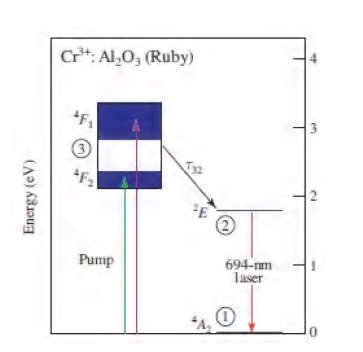
\includegraphics[width=0.75\linewidth]{Images/ruby.png}
    \caption{Relevant energy levels for operation of the ruby laser amplifier in the red. Stimulated emission on the transition from level 2 to 1 level gives rise to the wellknown red laser light~\cite{Saleh2007}.}
    \label{fig:ruby}
\end{figure}

Ruby is a dielectric medium with a refractive index \(n \approx 1.76\), composed of sapphire (\(\text{Al}_2\text{O}_3\)) doped with chromium ions (\(\text{Cr}^{3+}\)), which replace approximately \(0.05\%\) of the aluminum ions. Ruby was the first material to demonstrate laser action, though it is now rarely used and primarily serves as a didactic example~\cite{Saleh2007}.

Stimulated emission in ruby occurs across several transitions, with the well-known ruby-red laser radiation operating at \(\lambda_0 = 694.3 \, \text{nm}\). The system relies on a three-level pumping scheme (presented in Figure~\ref{fig:ruby}):
%
\begin{itemize}
  \item \textbf{Level 1:} The ground state and lower laser level.
  \item \textbf{Level 2:} The upper laser level, comprising two closely spaced sublevels ($R_1$ and $R_2$) responsible for the 694.3 nm emission.
  \item \textbf{Level 3:} Comprises two broad pump bands, centered in the green and violet. These serve to populate the upper and lower sublevels $R_2$ and $R_1$ of level 2, respectively (not resolved at the scale of the figure). The ruby's reddish color results from absorption in the pump bands when white light passes through it.
\end{itemize}
%

\subsubsection{\textbf{Pumping configurations}}
Ruby lasers are optically pumped using flashlamps:
\begin{itemize}
  \item \textbf{Helical flashlamp:} Surrounds the ruby rod for pumping (like in Figure~\ref{fig:pumping_techniques} (c)).
  \item \textbf{Elliptical configuration:} A more efficient setup where the ruby rod and a linear flashlamp are placed at the foci of a reflective cylinder with an elliptical cross-section.
\end{itemize}
A pulse of white light from the flashlamp excites \(\text{Cr}^{3+}\) ions in level 3, which rapidly decay to level 2 ($\tau_{32} \sim \text{ps}$), enabling stimulated emission. The excited ions remain in level 2
for a substantial period of time since the transition lifetime to level 1
is relatively long (nonradiative decay is negligible so that $\tau_21 \approx t_{sp}$). The ruby-laser system therefore complies with the three-level time-constant requirements dictated by Equation~\eqref{eq:results_three}.

The transition has a homogeneously broadened linewidth \(\Delta \nu \approx 330 \, \text{GHz}\) that arises principally from elastic electron scattering from lattice vibrations (phonons). The typical gain for a ruby laser is $\gamma(\nu)~\sim~1~\text{cm}^{-1}$~\cite{Koechner2010}.

\subsubsection{\textbf{Applications}}
Ruby lasers, though largely replaced by more efficient laser systems, are still used in specific applications where their unique characteristics are advantageous. Some notable applications include:
\begin{itemize}
  \item \textit{Holography:} The high coherence length and stability of the ruby laser's \(694.3 \, \text{nm}\) red light make it well-suited for producing high-quality holograms.
  \item \textit{Material processing:} Ruby lasers are used in specific material processing tasks, such as drilling, cutting, and engraving, where precise, high-intensity pulses are required.
  \item \textit{Scientific research:} Ruby lasers are mostly used as a didactic example in laser physics education and for experimental studies in optics and photonics.
\end{itemize}


\subsection{\textbf{Near-infrared region}}

If we go to higher wavelenghts, we find the near-infrared region ($\lambda \sim 700 \, \text{nm} - 2 \, \mu\text{m}$). In this region, the most used lasers available are Nd:YAG lasers ($1064 \, \text{nm}$) and semiconductor diode lasers ($800 \, \text{nm} - 1550 \, \text{nm}$).

\subsubsection{\textbf{Nd:YAG laser}}
These lasers are based on neodymium-doped yttrium aluminum garnet (YAG), a crystalline material with a high refractive index of approximately \( n \approx 1.82 \). Nd:YAG is widely recognized for its excellent thermal conductivity, high optical quality, and mechanical robustness, making it an ideal gain medium for both continuous-wave (CW) and high-repetition-rate pulsed lasers. The neodymium ion (Nd\(^{3+}\)) replaces a small fraction (typically \( < 1\% \)) of yttrium ions in the garnet crystal lattice, allowing efficient energy transfer while maintaining the structural integrity of the host~\cite{ndyag_lasers}.

The Nd:YAG laser operates as a four-level laser system:
\begin{itemize}
  \item \textbf{Level 0}: Ground state and lower laser level.
  \item \textbf{Level 1}: Short-lived energy level that lies above the ground state (negligible thermal population).
  \item \textbf{Level 2}: Metastable level responsible for stimulated emission.
  \item \textbf{Level 3}: Higher-energy pump level excited by pump sources.
\end{itemize}

Pumping is typically achieved using laser diodes, which efficiently excite ions from the ground state to the pump levels (centered near \( 808 \, \text{nm} \)). The excited ions rapidly decay to the metastable upper laser level, which has a spontaneous emission lifetime of \( t_{\text{sp}} \approx 230 \, \mu\text{s} \). Stimulated emission from level 2 to level 1 produces laser output at \( \lambda_0 = 1.064 \, \mu\text{m} \), in the near-infrared region.

\subsubsection{\textbf{Thermal and spectral properties}}
Nd:YAG has excellent thermal conductivity (\( \kappa \approx 14 \, \text{W/m·K} \)), allowing it to dissipate heat efficiently during high-power or continuous-wave operation. The short lifetime of the lower laser level (\( \tau_1 \approx 30 \, \text{ps} \)) and its significant energy gap (\( \Delta E \approx 0.2 \, \text{eV} \)) ensure negligible thermal population in level 1 at room temperature (\( kT \approx 0.026 \, \text{eV} \)).

Due to its crystalline nature, Nd:YAG exhibits a relatively narrow linewidth (\( \Delta\nu \approx 0.003 \, \text{nm} \)), which makes it ideal for applications requiring high beam quality, single-mode operation, and precise frequency control.

\subsubsection{\textbf{Applications}}
Nd:YAG lasers are one of the most versatile and widely used laser systems due to their reliability, efficiency, and scalability. Common applications include \textit{industrial manufacturing} (precision cutting, welding, and drilling), \textit{medical applications} (dermatology, ophthalmology, and laser surgery) and \textit{military use} (rangefinders and target designators).



\subsection{\textbf{Mid-infrared region}}
Moving to longer wavelengths, we find the mid-infrared region (\( \lambda \sim 2 \, \mu\text{m} - 20 \, \mu\text{m} \)). Among the most prominent lasers in this spectral region are the CO\textsubscript{2} lasers, which operate around \( 10.6 \, \mu\text{m} \).

\begin{figure}
    \centering
    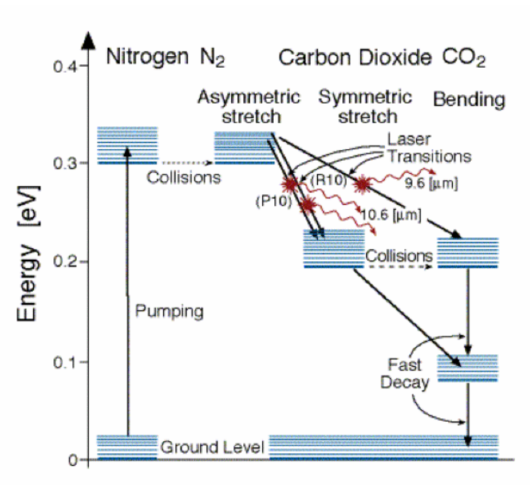
\includegraphics[width=\linewidth]{Images/CO2.png}
    \caption{Molecular laser system for a CO\textsubscript{2} laser~\cite{co2_lasers}.}
    \label{fig:CO2}
\end{figure}

\subsubsection{\textbf{CO\textsubscript{2} Laser}}
CO\textsubscript{2} lasers are gas lasers that utilize the vibrational and rotational transitions of carbon dioxide molecules to produce light in the mid-infrared region~\cite{co2_lasers}. These lasers are highly efficient and capable of producing continuous-wave (CW) or pulsed outputs with extremely high power levels. The lasing medium consists of a gas mixture, typically including CO\textsubscript{2}, nitrogen (N\textsubscript{2}), and helium (He), enclosed in a discharge tube.

The CO\textsubscript{2} laser operates as a molecular laser system (see Figure~\ref{fig:CO2}):
\begin{itemize}
  \item \textbf{Vibrational excitation}: Nitrogen molecules are excited by an electric discharge to their vibrational states, transferring energy to the CO\textsubscript{2} molecules via collisions.
  \item \textbf{Upper laser level}: The CO\textsubscript{2} molecules are excited to the asymmetric stretch vibrational mode (\( \nu_3 \)).
  \item \textbf{Laser transition}: Stimulated emission occurs as CO\textsubscript{2} transitions from the \( \nu_3 \) mode to the symmetric stretch (\( \nu_1 \)) or bending (\( \nu_2 \)) modes, emitting light at \( \lambda = 10.6 \, \mu\text{m} \).
  \item \textbf{Population inversion}: The helium atoms in the gas mixture help depopulate the lower laser levels, maintaining population inversion.
\end{itemize}

\subsubsection{\textbf{Thermal and spectral properties}}
CO\textsubscript{2} lasers are highly efficient~\cite{co2_lasers}, with conversion efficiencies reaching \( 20\% \), thanks to the effective energy transfer processes in the gas mixture. They produce narrow linewidths (\( \Delta\nu \approx 100 \, \text{MHz} \)) and high beam quality, making them suitable for applications requiring precise and focused infrared light. However, as gas lasers, they require cooling systems to manage heat dissipation during high-power operation.

\subsubsection{\textbf{Applications}}
CO\textsubscript{2} lasers are widely used in a variety of industries and research fields due to their power, efficiency, and versatility. Common applications include \textit{industrial manufacturing} (cutting, welding, drilling, and engraving of materials such as metals, plastics, and ceramics) and \textit{medical applications} (soft tissue surgery, dermatological procedures, and laser resurfacing).

\subsection{Far-infrared region}
In the far-infrared region (\( \lambda \sim 3 \, \mu\text{m} - 1 \, \text{mm} \)), the most widely used laser technology is the Quantum Cascade Laser (QCL). QCLs have revolutionized the far-infrared spectrum by enabling compact, tunable, and coherent light sources in this wavelength range. These lasers operate based on intersubband transitions in semiconductor materials and can cover a broad spectrum from the mid-infrared to the terahertz region.

\subsubsection{\textbf{Quantum Cascade Laser (QCL)}}
Quantum Cascade Lasers (QCLs) are based on semiconductor materials, typically composed of layers of materials such as indium gallium arsenide (InGaAs) or gallium arsenide (GaAs), arranged in quantum wells~\cite{qcl_lasers}. QCLs are designed to exploit intersubband transitions, which occur between discrete energy states within the conduction band of the semiconductor, unlike traditional lasers that rely on interband transitions.

\begin{figure}[!t]
    \centering
    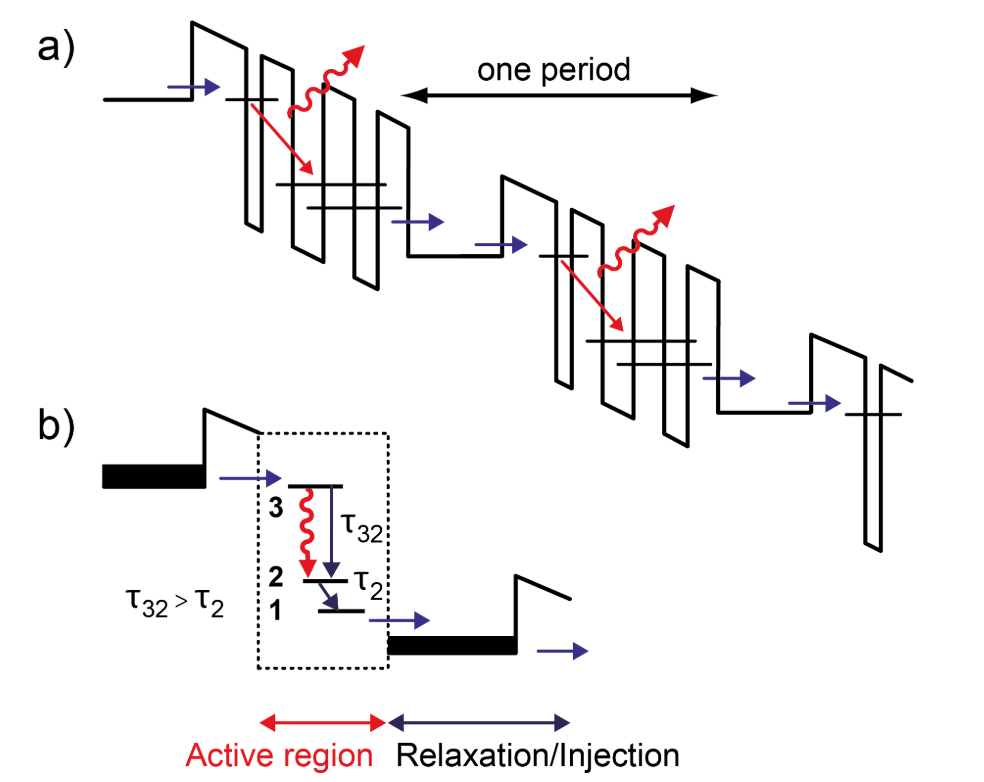
\includegraphics[width=1\linewidth]{Images/QCL.png}
    \caption{(a) Schematic of a conduction band diagram of a QCL. (b) Concept of the design of a QCL, where active region and relaxation/injection region are highlighted~\cite{qcl_lasers}.}
    \label{fig:QCL}
\end{figure}

The operating principle of the quantum cascade laser can be summarized as follows:

\begin{itemize}
    \item under the right applied bias, an electron will be injected via resonant tunneling in the upper state of the active region and relax to the lower state eventually emitting a photon.
    \item from here the electron will be transported through the relaxation region and then injected into the upper state of the following period where it will again be able to emit a photon.
    \item if the population inversion is ensured, as the current is increased gain will match the losses and the device will reach threshold, converting the injected electrons into photons by stimulated emission. The emitted power will depend linearly on the injected current.
\end{itemize}
In this way, each electron involved in the process can actually generate at most N photons, with N number of periods of the structure, when cascading across the structure. The process is repeated multiple times, creating a cascade effect that amplifies the output.

\subsubsection{\textbf{Thermal and spectral properties}}
QCLs are known for their excellent tunability and ability to emit in the far-infrared region, covering wavelengths from the mid-infrared to the terahertz region (\( 3 \, \mu\text{m} - 1 \, \text{mm} \)). The far-infrared wavelengths correspond to the lower photon energies (\( E \sim 1 - 10 \, \text{meV} \)) compared to visible or near-infrared lasers. This enables QCLs to be used in a variety of applications that require low-energy, long-wavelength radiation.

Due to their semiconductor nature, QCLs have a high efficiency in converting electrical power into optical power. They also exhibit low threshold current and can be designed for specific wavelength emissions by carefully engineering the quantum well structures. The spectral linewidth of QCLs is typically narrow (\( \Delta \nu \sim 1 - 5 \, \text{cm}^{-1} \)), making them suitable for precise spectroscopic measurements and sensing applications~\cite{qcl_lasers}.

The thermal management of QCLs is a key aspect of their performance; the lasers generate heat as a byproduct of the electrical pumping process, and efficient heat dissipation is critical for maintaining stable operation. Thermoelectric coolers or heat sinks are often used to keep the temperature within the optimal range.

\subsubsection{\textbf{Applications}}
Quantum Cascade Lasers are used in a variety of applications that require far-infrared or terahertz radiation. Some key areas of application include:
\begin{itemize}
  \item \textit{Spectroscopy and sensing}: QCLs are extensively used in molecular spectroscopy, where they provide high-resolution and tunable light sources for detecting gases and chemical compounds.
  \item \textit{Chemical and environmental sensing}: Due to their ability to emit at wavelengths corresponding to the absorption lines of various molecules (such as carbon dioxide, methane, and water vapor), QCLs are utilized in environmental monitoring and chemical detection.
  \item \textit{Security and defense}: QCLs are used in applications such as trace detection and imaging systems for security and defense purposes, particularly for detecting explosives or hazardous materials.
  \item \textit{Terahertz imaging}: QCLs emitting in the terahertz range are used in non-destructive testing, medical imaging, and security screening.
\end{itemize}

\section*{References}
\begin{thebibliography}{99}

\bibitem{Saleh2007}
Saleh B. E. A. \& Teich M. C., \textit{Fundamentals of Photonics}, Wiley (2007).

\bibitem{Siegman1986}
Siegman A. E., \textit{Lasers}, University Science Books (1986).

\bibitem{Milonni2010}
Milonni P. W. \& Eberly J. H., \textit{Laser Physics}, Wiley (2010).

\bibitem{optical_pumping}
H. H. S. Tsien, \textit{Optical Pumping: Fundamentals and Applications}, Cambridge University Press, 1981.

\bibitem{electrical_pumping}
M. S. Ketterle, W. Ketterle, and D. P. Boston, \textit{Electrical Pumping of Semiconductor Lasers}, IEEE Journal of Quantum Electronics, 1986, \textbf{22}, 11.

\bibitem{nuclear_pumping}
J. A. Pople, \textit{Nuclear Pumping in Laser Systems}, Oxford University Press, 1990.

\bibitem{chemical_pumping}
P. L. Richards, \textit{Chemical Pumping and Its Application to Laser Systems}, Journal of Applied Physics, 1982, \textbf{53}, 4, 2945-2953.

\bibitem{Coldren2012}
Coldren L. A., Corzine S. W. \& Mašović M. L., \textit{Diode Lasers and Photonic Integrated Circuits}, Wiley (2012).

\bibitem{Koechner2010}
Koechner W. \& Bass M., \textit{Solid-State Lasers: A Graduate Text}, Springer (2010).

\bibitem{nitrogen_lasers}
S. P. McGlynn, R. A. Cline, and R. G. W. Brown, \textit{Nitrogen Lasers: Theory and Practice}, Wiley-Interscience, 1975.

\bibitem{ndyag_lasers}
J. L. D. Meek, \textit{Nd:YAG Lasers: Fundamentals and Applications}, Springer, 1992.

\bibitem{co2_lasers}
E. D. C. Parker, \textit{CO\textsubscript{2} Lasers: Theory and Practice}, John Wiley \& Sons, 1972.

\bibitem{qcl_lasers}
J. Faist, F. Capasso, D. L. Sivco, C. R. Becker, and A. Y. Cho, \textit{Quantum Cascade Laser}, Science, 1994, \textbf{264}, 553-556.

\end{thebibliography}

\end{document}

